\documentclass[1p]{elsarticle_modified}
%\bibliographystyle{elsarticle-num}

%\usepackage[colorlinks]{hyperref}
%\usepackage{abbrmath_seonhwa} %\Abb, \Ascr, \Acal ,\Abf, \Afrak
\usepackage{amsfonts}
\usepackage{amssymb}
\usepackage{amsmath}
\usepackage{amsthm}
\usepackage{scalefnt}
\usepackage{amsbsy}
\usepackage{kotex}
\usepackage{caption}
\usepackage{subfig}
\usepackage{color}
\usepackage{graphicx}
\usepackage{xcolor} %% white, black, red, green, blue, cyan, magenta, yellow
\usepackage{float}
\usepackage{setspace}
\usepackage{hyperref}

\usepackage{tikz}
\usetikzlibrary{arrows}

\usepackage{multirow}
\usepackage{array} % fixed length table
\usepackage{hhline}

%%%%%%%%%%%%%%%%%%%%%
\makeatletter
\renewcommand*\env@matrix[1][\arraystretch]{%
	\edef\arraystretch{#1}%
	\hskip -\arraycolsep
	\let\@ifnextchar\new@ifnextchar
	\array{*\c@MaxMatrixCols c}}
\makeatother %https://tex.stackexchange.com/questions/14071/how-can-i-increase-the-line-spacing-in-a-matrix
%%%%%%%%%%%%%%%

\usepackage[normalem]{ulem}

\newcommand{\msout}[1]{\ifmmode\text{\sout{\ensuremath{#1}}}\else\sout{#1}\fi}
%SOURCE: \msout is \stkout macro in https://tex.stackexchange.com/questions/20609/strikeout-in-math-mode

\newcommand{\cancel}[1]{
	\ifmmode
	{\color{red}\msout{#1}}
	\else
	{\color{red}\sout{#1}}
	\fi
}

\newcommand{\add}[1]{
	{\color{blue}\uwave{#1}}
}

\newcommand{\replace}[2]{
	\ifmmode
	{\color{red}\msout{#1}}{\color{blue}\uwave{#2}}
	\else
	{\color{red}\sout{#1}}{\color{blue}\uwave{#2}}
	\fi
}

\newcommand{\Sol}{\mathcal{S}} %segment
\newcommand{\D}{D} %diagram
\newcommand{\A}{\mathcal{A}} %arc


%%%%%%%%%%%%%%%%%%%%%%%%%%%%%5 test

\def\sl{\operatorname{\textup{SL}}(2,\Cbb)}
\def\psl{\operatorname{\textup{PSL}}(2,\Cbb)}
\def\quan{\mkern 1mu \triangleright \mkern 1mu}

\theoremstyle{definition}
\newtheorem{thm}{Theorem}[section]
\newtheorem{prop}[thm]{Proposition}
\newtheorem{lem}[thm]{Lemma}
\newtheorem{ques}[thm]{Question}
\newtheorem{cor}[thm]{Corollary}
\newtheorem{defn}[thm]{Definition}
\newtheorem{exam}[thm]{Example}
\newtheorem{rmk}[thm]{Remark}
\newtheorem{alg}[thm]{Algorithm}

\newcommand{\I}{\sqrt{-1}}
\begin{document}

%\begin{frontmatter}
%
%\title{Boundary parabolic representations of knots up to 8 crossings}
%
%%% Group authors per affiliation:
%\author{Yunhi Cho} 
%\address{Department of Mathematics, University of Seoul, Seoul, Korea}
%\ead{yhcho@uos.ac.kr}
%
%
%\author{Seonhwa Kim} %\fnref{s_kim}}
%\address{Center for Geometry and Physics, Institute for Basic Science, Pohang, 37673, Korea}
%\ead{ryeona17@ibs.re.kr}
%
%\author{Hyuk Kim}
%\address{Department of Mathematical Sciences, Seoul National University, Seoul 08826, Korea}
%\ead{hyukkim@snu.ac.kr}
%
%\author{Seokbeom Yoon}
%\address{Department of Mathematical Sciences, Seoul National University, Seoul, 08826,  Korea}
%\ead{sbyoon15@snu.ac.kr}
%
%\begin{abstract}
%We find all boundary parabolic representation of knots up to 8 crossings.
%
%\end{abstract}
%\begin{keyword}
%    \MSC[2010] 57M25 
%\end{keyword}
%
%\end{frontmatter}

%\linenumbers
%\tableofcontents
%
\newcommand\colored[1]{\textcolor{white}{\rule[-0.35ex]{0.8em}{1.4ex}}\kern-0.8em\color{red} #1}%
%\newcommand\colored[1]{\textcolor{white}{ #1}\kern-2.17ex	\textcolor{white}{ #1}\kern-1.81ex	\textcolor{white}{ #1}\kern-2.15ex\color{red}#1	}

{\Large $\underline{12a_{1087}~(K12a_{1087})}$}

\setlength{\tabcolsep}{10pt}
\renewcommand{\arraystretch}{1.6}
\vspace{1cm}\begin{tabular}{m{100pt}>{\centering\arraybackslash}m{274pt}}
\multirow{5}{120pt}{
	\centering
	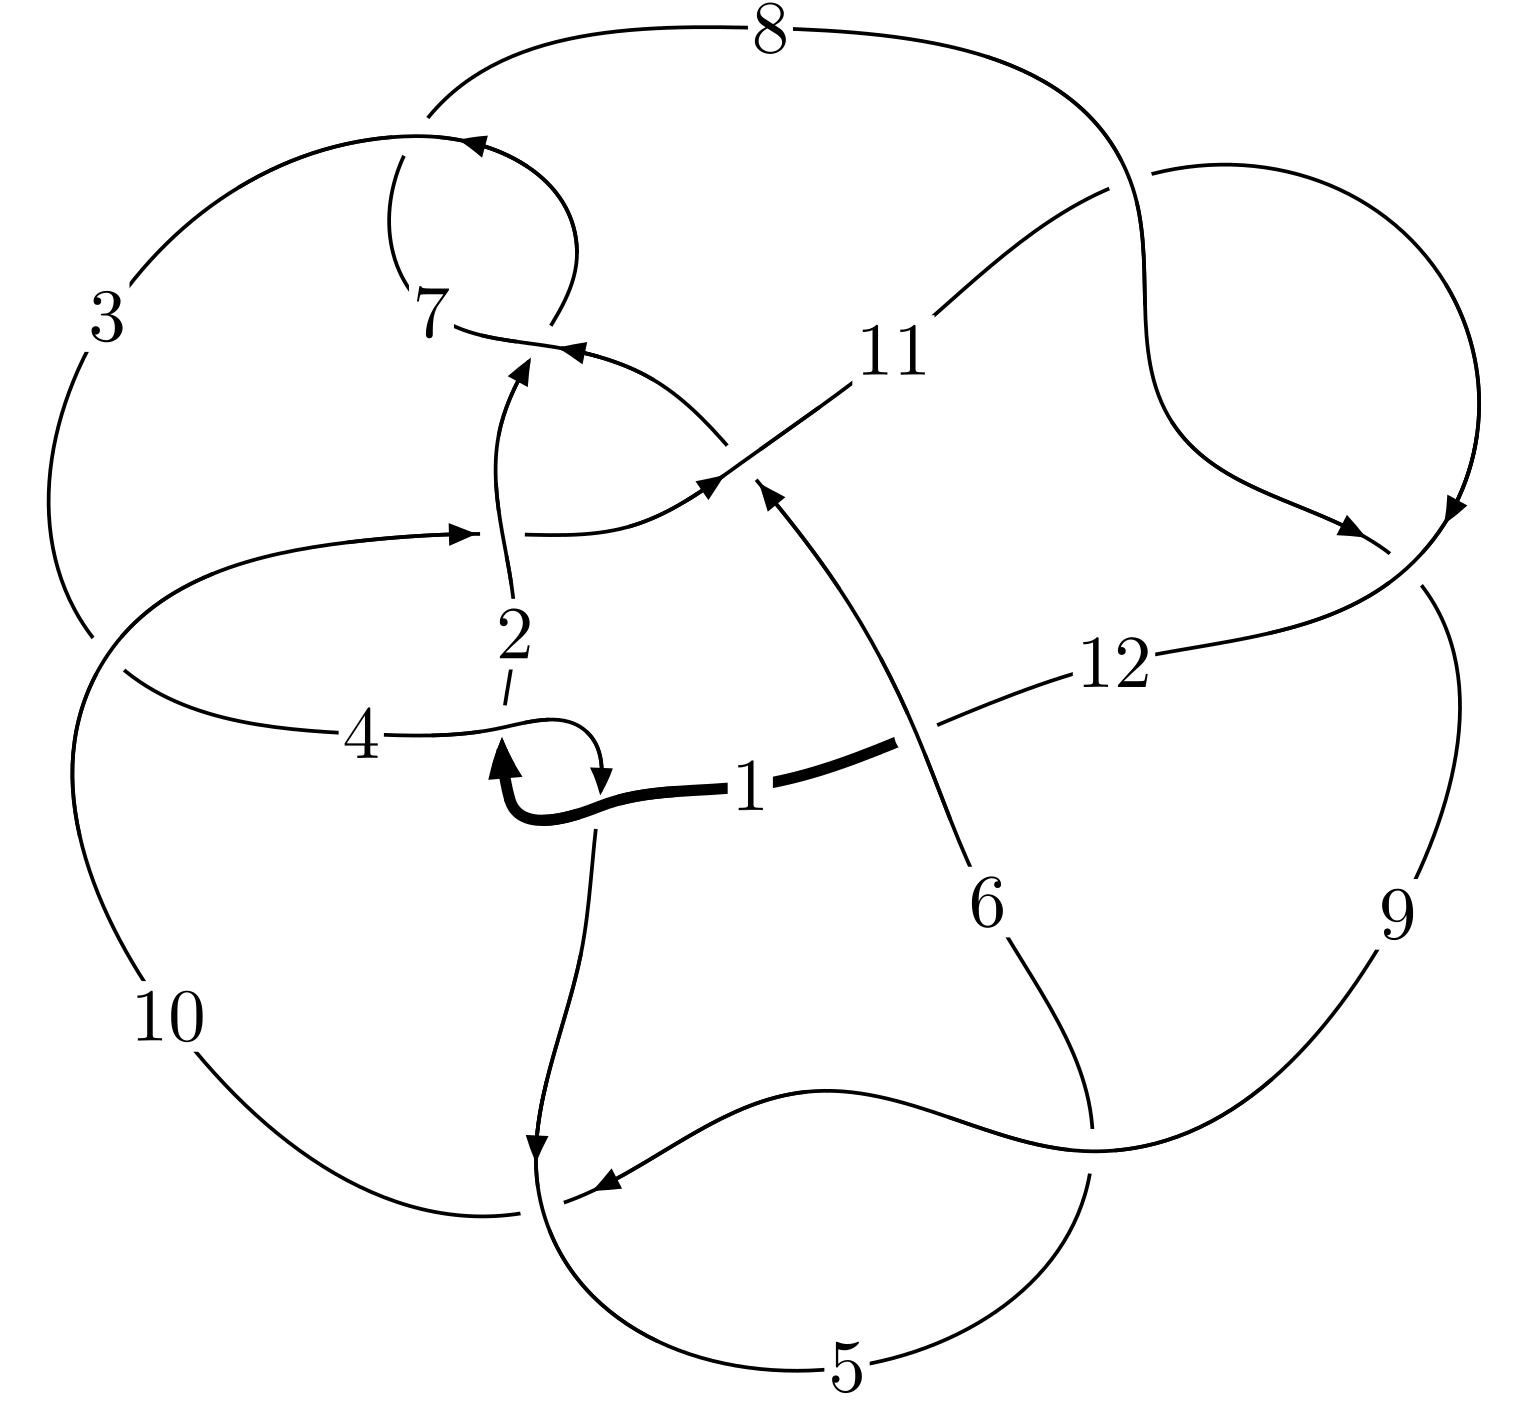
\includegraphics[width=112pt]{../../../GIT/diagram.site/Diagrams/png/1888_12a_1087.png}\\
\ \ \ A knot diagram\footnotemark}&
\allowdisplaybreaks
\textbf{Linearized knot diagam} \\
\cline{2-2}
 &
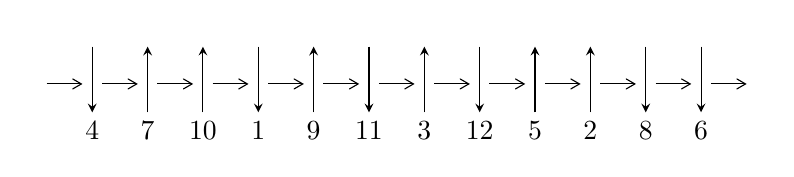
\begin{tikzpicture}[x=20pt, y=17pt]
	% nodes
	\node (C0) at (0, 0) {};
	\node (C1) at (1, 0) {};
	\node (C1U) at (1, +1) {};
	\node (C1D) at (1, -1) {4};

	\node (C2) at (2, 0) {};
	\node (C2U) at (2, +1) {};
	\node (C2D) at (2, -1) {7};

	\node (C3) at (3, 0) {};
	\node (C3U) at (3, +1) {};
	\node (C3D) at (3, -1) {10};

	\node (C4) at (4, 0) {};
	\node (C4U) at (4, +1) {};
	\node (C4D) at (4, -1) {1};

	\node (C5) at (5, 0) {};
	\node (C5U) at (5, +1) {};
	\node (C5D) at (5, -1) {9};

	\node (C6) at (6, 0) {};
	\node (C6U) at (6, +1) {};
	\node (C6D) at (6, -1) {11};

	\node (C7) at (7, 0) {};
	\node (C7U) at (7, +1) {};
	\node (C7D) at (7, -1) {3};

	\node (C8) at (8, 0) {};
	\node (C8U) at (8, +1) {};
	\node (C8D) at (8, -1) {12};

	\node (C9) at (9, 0) {};
	\node (C9U) at (9, +1) {};
	\node (C9D) at (9, -1) {5};

	\node (C10) at (10, 0) {};
	\node (C10U) at (10, +1) {};
	\node (C10D) at (10, -1) {2};

	\node (C11) at (11, 0) {};
	\node (C11U) at (11, +1) {};
	\node (C11D) at (11, -1) {8};

	\node (C12) at (12, 0) {};
	\node (C12U) at (12, +1) {};
	\node (C12D) at (12, -1) {6};
	\node (C13) at (13, 0) {};

	% arrows
	\draw[->,>={angle 60}]
	(C0) edge (C1) (C1) edge (C2) (C2) edge (C3) (C3) edge (C4) (C4) edge (C5) (C5) edge (C6) (C6) edge (C7) (C7) edge (C8) (C8) edge (C9) (C9) edge (C10) (C10) edge (C11) (C11) edge (C12) (C12) edge (C13) ;	\draw[->,>=stealth]
	(C1U) edge (C1D) (C2D) edge (C2U) (C3D) edge (C3U) (C4U) edge (C4D) (C5D) edge (C5U) (C6U) edge (C6D) (C7D) edge (C7U) (C8U) edge (C8D) (C9D) edge (C9U) (C10D) edge (C10U) (C11U) edge (C11D) (C12U) edge (C12D) ;
	\end{tikzpicture} \\
\hhline{~~} \\& 
\textbf{Solving Sequence} \\ \cline{2-2} 
 &
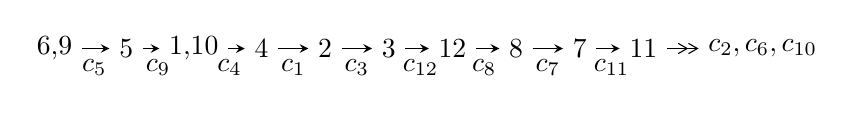
\begin{tikzpicture}[x=23pt, y=7pt]
	% node
	\node (A0) at (-1/8, 0) {6,9};
	\node (A1) at (1, 0) {5};
	\node (A2) at (33/16, 0) {1,10};
	\node (A3) at (25/8, 0) {4};
	\node (A4) at (33/8, 0) {2};
	\node (A5) at (41/8, 0) {3};
	\node (A6) at (49/8, 0) {12};
	\node (A7) at (57/8, 0) {8};
	\node (A8) at (65/8, 0) {7};
	\node (A9) at (73/8, 0) {11};
	\node (C1) at (1/2, -1) {$c_{5}$};
	\node (C2) at (3/2, -1) {$c_{9}$};
	\node (C3) at (21/8, -1) {$c_{4}$};
	\node (C4) at (29/8, -1) {$c_{1}$};
	\node (C5) at (37/8, -1) {$c_{3}$};
	\node (C6) at (45/8, -1) {$c_{12}$};
	\node (C7) at (53/8, -1) {$c_{8}$};
	\node (C8) at (61/8, -1) {$c_{7}$};
	\node (C9) at (69/8, -1) {$c_{11}$};
	\node (A10) at (11, 0) {$c_{2},c_{6},c_{10}$};

	% edge
	\draw[->,>=stealth]	
	(A0) edge (A1) (A1) edge (A2) (A2) edge (A3) (A3) edge (A4) (A4) edge (A5) (A5) edge (A6) (A6) edge (A7) (A7) edge (A8) (A8) edge (A9) ;
	\draw[->>,>={angle 60}]	
	(A9) edge (A10);
\end{tikzpicture} \\ 

\end{tabular} \\

\footnotetext{
The image of knot diagram is generated by the software ``\textbf{Draw programme}" developed by Andrew Bartholomew(\url{http://www.layer8.co.uk/maths/draw/index.htm\#Running-draw}), where we modified some parts for our purpose(\url{https://github.com/CATsTAILs/LinksPainter}).
}\phantom \\ \newline 
\centering \textbf{Ideals for irreducible components\footnotemark of $X_{\text{par}}$} 
 
\begin{align*}
I^u_{1}&=\langle 
1.91910\times10^{765} u^{138}+3.12076\times10^{766} u^{137}+\cdots+2.08048\times10^{766} b-1.92264\times10^{769},\\
\phantom{I^u_{1}}&\phantom{= \langle  }-2.36640\times10^{768} u^{138}-3.49494\times10^{769} u^{137}+\cdots+2.56107\times10^{769} a+1.97863\times10^{772},\\
\phantom{I^u_{1}}&\phantom{= \langle  }u^{139}+7 u^{138}+\cdots+11682 u-1231\rangle \\
I^u_{2}&=\langle 
-1.20250\times10^{21} u^{26}-3.96564\times10^{20} u^{25}+\cdots+3.82872\times10^{21} b-2.56885\times10^{21},\\
\phantom{I^u_{2}}&\phantom{= \langle  }1.83911\times10^{22} u^{26}+3.24467\times10^{22} u^{25}+\cdots+3.82872\times10^{21} a+2.71471\times10^{22},\;u^{27}+2 u^{26}+\cdots+2 u-1\rangle \\
\\
\end{align*}
\raggedright * 2 irreducible components of $\dim_{\mathbb{C}}=0$, with total 166 representations.\\
\footnotetext{All coefficients of polynomials are rational numbers. But the coefficients are sometimes approximated in decimal forms when there is not enough margin.}
\newpage
\renewcommand{\arraystretch}{1}
\centering \section*{I. $I^u_{1}= \langle 1.92\times10^{765} u^{138}+3.12\times10^{766} u^{137}+\cdots+2.08\times10^{766} b-1.92\times10^{769},\;-2.37\times10^{768} u^{138}-3.49\times10^{769} u^{137}+\cdots+2.56\times10^{769} a+1.98\times10^{772},\;u^{139}+7 u^{138}+\cdots+11682 u-1231 \rangle$}
\flushleft \textbf{(i) Arc colorings}\\
\begin{tabular}{m{7pt} m{180pt} m{7pt} m{180pt} }
\flushright $a_{6}=$&$\begin{pmatrix}1\\0\end{pmatrix}$ \\
\flushright $a_{9}=$&$\begin{pmatrix}0\\u\end{pmatrix}$ \\
\flushright $a_{5}=$&$\begin{pmatrix}1\\u^2\end{pmatrix}$ \\
\flushright $a_{1}=$&$\begin{pmatrix}0.0923992 u^{138}+1.36464 u^{137}+\cdots+7209.45 u-772.579\\-0.0922435 u^{138}-1.50002 u^{137}+\cdots-8590.71 u+924.136\end{pmatrix}$ \\
\flushright $a_{10}=$&$\begin{pmatrix}u\\u^3+u\end{pmatrix}$ \\
\flushright $a_{4}=$&$\begin{pmatrix}-0.549881 u^{138}-3.93080 u^{137}+\cdots-52.9648 u+59.9517\\0.399436 u^{138}+2.81424 u^{137}+\cdots-390.909 u-0.625575\end{pmatrix}$ \\
\flushright $a_{2}=$&$\begin{pmatrix}0.225887 u^{138}+1.40797 u^{137}+\cdots-2060.40 u+193.283\\-0.0274120 u^{138}-0.225529 u^{137}+\cdots-219.675 u+30.6034\end{pmatrix}$ \\
\flushright $a_{3}=$&$\begin{pmatrix}-0.189124 u^{138}-1.42316 u^{137}+\cdots-713.671 u+93.3319\\0.310659 u^{138}+2.17704 u^{137}+\cdots-401.163 u+11.0094\end{pmatrix}$ \\
\flushright $a_{12}=$&$\begin{pmatrix}0.000155686 u^{138}-0.135379 u^{137}+\cdots-1381.27 u+151.556\\-0.0922435 u^{138}-1.50002 u^{137}+\cdots-8590.71 u+924.136\end{pmatrix}$ \\
\flushright $a_{8}=$&$\begin{pmatrix}0.0441154 u^{138}+0.262529 u^{137}+\cdots-450.945 u+42.2162\\-0.0738248 u^{138}-0.0284938 u^{137}+\cdots+4575.07 u-472.844\end{pmatrix}$ \\
\flushright $a_{7}=$&$\begin{pmatrix}0.0177352 u^{138}-0.0819765 u^{137}+\cdots-2406.75 u+251.185\\0.355643 u^{138}+2.56097 u^{137}+\cdots+163.686 u-59.8001\end{pmatrix}$ \\
\flushright $a_{11}=$&$\begin{pmatrix}-0.0205174 u^{138}-0.0898126 u^{137}+\cdots+597.154 u-56.9696\\-0.0652540 u^{138}-0.245445 u^{137}+\cdots+2278.61 u-233.997\end{pmatrix}$\\&\end{tabular}
\flushleft \textbf{(ii) Obstruction class $= -1$}\\~\\
\flushleft \textbf{(iii) Cusp Shapes $= 1.43120 u^{138}+9.34049 u^{137}+\cdots-9490.61 u+842.501$}\\~\\
\newpage\renewcommand{\arraystretch}{1}
\flushleft \textbf{(iv) u-Polynomials at the component}\newline \\
\begin{tabular}{m{50pt}|m{274pt}}
Crossings & \hspace{64pt}u-Polynomials at each crossing \\
\hline $$\begin{aligned}c_{1},c_{4}\end{aligned}$$&$\begin{aligned}
&u^{139}-8 u^{138}+\cdots+16402 u-877
\end{aligned}$\\
\hline $$\begin{aligned}c_{2},c_{7}\end{aligned}$$&$\begin{aligned}
&u^{139}+u^{138}+\cdots-2696 u+400
\end{aligned}$\\
\hline $$\begin{aligned}c_{3}\end{aligned}$$&$\begin{aligned}
&u^{139}+u^{138}+\cdots+8317 u-739
\end{aligned}$\\
\hline $$\begin{aligned}c_{5},c_{9}\end{aligned}$$&$\begin{aligned}
&u^{139}-7 u^{138}+\cdots+11682 u+1231
\end{aligned}$\\
\hline $$\begin{aligned}c_{6}\end{aligned}$$&$\begin{aligned}
&u^{139}-5 u^{138}+\cdots+3449844 u+1329092
\end{aligned}$\\
\hline $$\begin{aligned}c_{8},c_{11}\end{aligned}$$&$\begin{aligned}
&u^{139}-53 u^{137}+\cdots+347585 u+14407
\end{aligned}$\\
\hline $$\begin{aligned}c_{10}\end{aligned}$$&$\begin{aligned}
&u^{139}+u^{138}+\cdots-2613392 u+228149
\end{aligned}$\\
\hline $$\begin{aligned}c_{12}\end{aligned}$$&$\begin{aligned}
&u^{139}+2 u^{138}+\cdots-1050507 u-108932
\end{aligned}$\\
\hline
\end{tabular}\\~\\
\newpage\renewcommand{\arraystretch}{1}
\flushleft \textbf{(v) Riley Polynomials at the component}\newline \\
\begin{tabular}{m{50pt}|m{274pt}}
Crossings & \hspace{64pt}Riley Polynomials at each crossing \\
\hline $$\begin{aligned}c_{1},c_{4}\end{aligned}$$&$\begin{aligned}
&y^{139}+92 y^{138}+\cdots-1895482 y-769129
\end{aligned}$\\
\hline $$\begin{aligned}c_{2},c_{7}\end{aligned}$$&$\begin{aligned}
&y^{139}-75 y^{138}+\cdots+7284416 y-160000
\end{aligned}$\\
\hline $$\begin{aligned}c_{3}\end{aligned}$$&$\begin{aligned}
&y^{139}-7 y^{138}+\cdots+158245637 y-546121
\end{aligned}$\\
\hline $$\begin{aligned}c_{5},c_{9}\end{aligned}$$&$\begin{aligned}
&y^{139}+111 y^{138}+\cdots-54973534 y-1515361
\end{aligned}$\\
\hline $$\begin{aligned}c_{6}\end{aligned}$$&$\begin{aligned}
&y^{139}+33 y^{138}+\cdots-63550645426176 y-1766485544464
\end{aligned}$\\
\hline $$\begin{aligned}c_{8},c_{11}\end{aligned}$$&$\begin{aligned}
&y^{139}-106 y^{138}+\cdots+5626584101 y-207561649
\end{aligned}$\\
\hline $$\begin{aligned}c_{10}\end{aligned}$$&$\begin{aligned}
&y^{139}-61 y^{138}+\cdots+6848256291546 y-52051966201
\end{aligned}$\\
\hline $$\begin{aligned}c_{12}\end{aligned}$$&$\begin{aligned}
&y^{139}-34 y^{138}+\cdots+547581039921 y-11866180624
\end{aligned}$\\
\hline
\end{tabular}\\~\\
\newpage\flushleft \textbf{(vi) Complex Volumes and Cusp Shapes}
$$\begin{array}{c|c|c}  
\text{Solutions to }I^u_{1}& \I (\text{vol} + \sqrt{-1}CS) & \text{Cusp shape}\\
 \hline 
\begin{aligned}
u &= -0.039989 + 1.017880 I \\
a &= \phantom{-}0.0196678 - 0.0235319 I \\
b &= \phantom{-}0.03432 - 1.63507 I\end{aligned}
 & \phantom{-}1.36706 - 0.77225 I & \phantom{-0.000000 } 0 \\ \hline\begin{aligned}
u &= -0.039989 - 1.017880 I \\
a &= \phantom{-}0.0196678 + 0.0235319 I \\
b &= \phantom{-}0.03432 + 1.63507 I\end{aligned}
 & \phantom{-}1.36706 + 0.77225 I & \phantom{-0.000000 } 0 \\ \hline\begin{aligned}
u &= \phantom{-}0.481191 + 0.937078 I \\
a &= \phantom{-}1.67515 + 0.27171 I \\
b &= -0.519513 + 0.402886 I\end{aligned}
 & \phantom{-}0.23466 + 4.83606 I & \phantom{-0.000000 } 0 \\ \hline\begin{aligned}
u &= \phantom{-}0.481191 - 0.937078 I \\
a &= \phantom{-}1.67515 - 0.27171 I \\
b &= -0.519513 - 0.402886 I\end{aligned}
 & \phantom{-}0.23466 - 4.83606 I & \phantom{-0.000000 } 0 \\ \hline\begin{aligned}
u &= -0.942337 + 0.076060 I \\
a &= -0.331531 - 0.494964 I \\
b &= -0.686624 + 0.904248 I\end{aligned}
 & \phantom{-}7.02740 + 3.30222 I & \phantom{-0.000000 } 0 \\ \hline\begin{aligned}
u &= -0.942337 - 0.076060 I \\
a &= -0.331531 + 0.494964 I \\
b &= -0.686624 - 0.904248 I\end{aligned}
 & \phantom{-}7.02740 - 3.30222 I & \phantom{-0.000000 } 0 \\ \hline\begin{aligned}
u &= -0.939126 + 0.062489 I \\
a &= -0.180705 + 0.241630 I \\
b &= \phantom{-}0.143026 - 1.053040 I\end{aligned}
 & \phantom{-}4.84217 + 3.09296 I & \phantom{-0.000000 } 0 \\ \hline\begin{aligned}
u &= -0.939126 - 0.062489 I \\
a &= -0.180705 - 0.241630 I \\
b &= \phantom{-}0.143026 + 1.053040 I\end{aligned}
 & \phantom{-}4.84217 - 3.09296 I & \phantom{-0.000000 } 0 \\ \hline\begin{aligned}
u &= \phantom{-}0.182420 + 1.045360 I \\
a &= -1.82996 - 0.34133 I \\
b &= \phantom{-}0.438713 - 0.455038 I\end{aligned}
 & \phantom{-}0.96021 + 6.14982 I & \phantom{-0.000000 } 0 \\ \hline\begin{aligned}
u &= \phantom{-}0.182420 - 1.045360 I \\
a &= -1.82996 + 0.34133 I \\
b &= \phantom{-}0.438713 + 0.455038 I\end{aligned}
 & \phantom{-}0.96021 - 6.14982 I & \phantom{-0.000000 } 0\\
 \hline 
 \end{array}$$\newpage$$\begin{array}{c|c|c}  
\text{Solutions to }I^u_{1}& \I (\text{vol} + \sqrt{-1}CS) & \text{Cusp shape}\\
 \hline 
\begin{aligned}
u &= \phantom{-}1.031760 + 0.257231 I \\
a &= \phantom{-}0.146884 + 0.150541 I \\
b &= -0.308572 - 1.066430 I\end{aligned}
 & \phantom{-}8.12766 - 7.82410 I & \phantom{-0.000000 } 0 \\ \hline\begin{aligned}
u &= \phantom{-}1.031760 - 0.257231 I \\
a &= \phantom{-}0.146884 - 0.150541 I \\
b &= -0.308572 + 1.066430 I\end{aligned}
 & \phantom{-}8.12766 + 7.82410 I & \phantom{-0.000000 } 0 \\ \hline\begin{aligned}
u &= \phantom{-}0.087117 + 1.060770 I \\
a &= -1.66253 + 0.22246 I \\
b &= \phantom{-}1.63686 - 1.46324 I\end{aligned}
 & -4.75228 + 2.50216 I & \phantom{-0.000000 } 0 \\ \hline\begin{aligned}
u &= \phantom{-}0.087117 - 1.060770 I \\
a &= -1.66253 - 0.22246 I \\
b &= \phantom{-}1.63686 + 1.46324 I\end{aligned}
 & -4.75228 - 2.50216 I & \phantom{-0.000000 } 0 \\ \hline\begin{aligned}
u &= \phantom{-}0.590045 + 0.721712 I \\
a &= -0.134505 + 0.309103 I \\
b &= \phantom{-}0.150663 + 0.635932 I\end{aligned}
 & \phantom{-}0.992305 - 0.435783 I & \phantom{-0.000000 } 0 \\ \hline\begin{aligned}
u &= \phantom{-}0.590045 - 0.721712 I \\
a &= -0.134505 - 0.309103 I \\
b &= \phantom{-}0.150663 - 0.635932 I\end{aligned}
 & \phantom{-}0.992305 + 0.435783 I & \phantom{-0.000000 } 0 \\ \hline\begin{aligned}
u &= \phantom{-}0.031384 + 1.076740 I \\
a &= -2.33667 - 0.43733 I \\
b &= \phantom{-}2.35961 + 1.54533 I\end{aligned}
 & -0.42394 + 8.03187 I & \phantom{-0.000000 } 0 \\ \hline\begin{aligned}
u &= \phantom{-}0.031384 - 1.076740 I \\
a &= -2.33667 + 0.43733 I \\
b &= \phantom{-}2.35961 - 1.54533 I\end{aligned}
 & -0.42394 - 8.03187 I & \phantom{-0.000000 } 0 \\ \hline\begin{aligned}
u &= -0.791917 + 0.453106 I \\
a &= \phantom{-}0.277654 + 1.369740 I \\
b &= \phantom{-}1.066170 - 0.918445 I\end{aligned}
 & \phantom{-}3.95818 + 3.42854 I & \phantom{-0.000000 } 0 \\ \hline\begin{aligned}
u &= -0.791917 - 0.453106 I \\
a &= \phantom{-}0.277654 - 1.369740 I \\
b &= \phantom{-}1.066170 + 0.918445 I\end{aligned}
 & \phantom{-}3.95818 - 3.42854 I & \phantom{-0.000000 } 0\\
 \hline 
 \end{array}$$\newpage$$\begin{array}{c|c|c}  
\text{Solutions to }I^u_{1}& \I (\text{vol} + \sqrt{-1}CS) & \text{Cusp shape}\\
 \hline 
\begin{aligned}
u &= \phantom{-}0.054450 + 1.088940 I \\
a &= \phantom{-}2.11968 + 0.67772 I \\
b &= -1.99435 + 0.39427 I\end{aligned}
 & -4.99290 - 1.46818 I & \phantom{-0.000000 } 0 \\ \hline\begin{aligned}
u &= \phantom{-}0.054450 - 1.088940 I \\
a &= \phantom{-}2.11968 - 0.67772 I \\
b &= -1.99435 - 0.39427 I\end{aligned}
 & -4.99290 + 1.46818 I & \phantom{-0.000000 } 0 \\ \hline\begin{aligned}
u &= -0.447675 + 0.789562 I \\
a &= \phantom{-}0.114568 + 0.948194 I \\
b &= \phantom{-}0.123171 + 0.921072 I\end{aligned}
 & \phantom{-}3.21263 + 2.15083 I & \phantom{-0.000000 } 0 \\ \hline\begin{aligned}
u &= -0.447675 - 0.789562 I \\
a &= \phantom{-}0.114568 - 0.948194 I \\
b &= \phantom{-}0.123171 - 0.921072 I\end{aligned}
 & \phantom{-}3.21263 - 2.15083 I & \phantom{-0.000000 } 0 \\ \hline\begin{aligned}
u &= \phantom{-}0.083801 + 1.099070 I \\
a &= \phantom{-}0.798809 + 0.207338 I \\
b &= -0.67844 - 1.34155 I\end{aligned}
 & -3.06633 + 3.30259 I & \phantom{-0.000000 } 0 \\ \hline\begin{aligned}
u &= \phantom{-}0.083801 - 1.099070 I \\
a &= \phantom{-}0.798809 - 0.207338 I \\
b &= -0.67844 + 1.34155 I\end{aligned}
 & -3.06633 - 3.30259 I & \phantom{-0.000000 } 0 \\ \hline\begin{aligned}
u &= -0.068937 + 0.892914 I \\
a &= \phantom{-}2.51879 - 1.17012 I \\
b &= -2.21428 - 0.26115 I\end{aligned}
 & \phantom{-}0.44041 - 8.05097 I & \phantom{-0.000000 } 0 \\ \hline\begin{aligned}
u &= -0.068937 - 0.892914 I \\
a &= \phantom{-}2.51879 + 1.17012 I \\
b &= -2.21428 + 0.26115 I\end{aligned}
 & \phantom{-}0.44041 + 8.05097 I & \phantom{-0.000000 } 0 \\ \hline\begin{aligned}
u &= -0.077678 + 0.890499 I \\
a &= \phantom{-}0.71200 + 1.71379 I \\
b &= -0.174279 - 0.279106 I\end{aligned}
 & \phantom{-}1.70213 + 0.28632 I & \phantom{-0.000000 } 0 \\ \hline\begin{aligned}
u &= -0.077678 - 0.890499 I \\
a &= \phantom{-}0.71200 - 1.71379 I \\
b &= -0.174279 + 0.279106 I\end{aligned}
 & \phantom{-}1.70213 - 0.28632 I & \phantom{-0.000000 } 0\\
 \hline 
 \end{array}$$\newpage$$\begin{array}{c|c|c}  
\text{Solutions to }I^u_{1}& \I (\text{vol} + \sqrt{-1}CS) & \text{Cusp shape}\\
 \hline 
\begin{aligned}
u &= -0.088786 + 1.106150 I \\
a &= -1.40345 + 1.03827 I \\
b &= \phantom{-}0.773931 + 0.572411 I\end{aligned}
 & -1.09142 - 5.55350 I & \phantom{-0.000000 } 0 \\ \hline\begin{aligned}
u &= -0.088786 - 1.106150 I \\
a &= -1.40345 - 1.03827 I \\
b &= \phantom{-}0.773931 - 0.572411 I\end{aligned}
 & -1.09142 + 5.55350 I & \phantom{-0.000000 } 0 \\ \hline\begin{aligned}
u &= \phantom{-}0.834045 + 0.273977 I \\
a &= -0.876904 - 0.079081 I \\
b &= -0.396614 + 0.757911 I\end{aligned}
 & \phantom{-}0.655785 + 0.412691 I & \phantom{-0.000000 } 0 \\ \hline\begin{aligned}
u &= \phantom{-}0.834045 - 0.273977 I \\
a &= -0.876904 + 0.079081 I \\
b &= -0.396614 - 0.757911 I\end{aligned}
 & \phantom{-}0.655785 - 0.412691 I & \phantom{-0.000000 } 0 \\ \hline\begin{aligned}
u &= -0.220109 + 0.849026 I \\
a &= -2.21359 - 0.53451 I \\
b &= \phantom{-}0.212927 - 0.037209 I\end{aligned}
 & \phantom{-}3.30502 - 5.19427 I & \phantom{-0.000000 } 0 \\ \hline\begin{aligned}
u &= -0.220109 - 0.849026 I \\
a &= -2.21359 + 0.53451 I \\
b &= \phantom{-}0.212927 + 0.037209 I\end{aligned}
 & \phantom{-}3.30502 + 5.19427 I & \phantom{-0.000000 } 0 \\ \hline\begin{aligned}
u &= \phantom{-}0.367380 + 1.077480 I \\
a &= \phantom{-}1.68645 - 0.77728 I \\
b &= -1.01153 + 1.01694 I\end{aligned}
 & \phantom{-}5.73298 + 3.93821 I & \phantom{-0.000000 } 0 \\ \hline\begin{aligned}
u &= \phantom{-}0.367380 - 1.077480 I \\
a &= \phantom{-}1.68645 + 0.77728 I \\
b &= -1.01153 - 1.01694 I\end{aligned}
 & \phantom{-}5.73298 - 3.93821 I & \phantom{-0.000000 } 0 \\ \hline\begin{aligned}
u &= -0.327601 + 1.090830 I \\
a &= -1.42439 + 0.51690 I \\
b &= \phantom{-}1.087470 + 0.507462 I\end{aligned}
 & -0.46130 - 3.27866 I & \phantom{-0.000000 } 0 \\ \hline\begin{aligned}
u &= -0.327601 - 1.090830 I \\
a &= -1.42439 - 0.51690 I \\
b &= \phantom{-}1.087470 - 0.507462 I\end{aligned}
 & -0.46130 + 3.27866 I & \phantom{-0.000000 } 0\\
 \hline 
 \end{array}$$\newpage$$\begin{array}{c|c|c}  
\text{Solutions to }I^u_{1}& \I (\text{vol} + \sqrt{-1}CS) & \text{Cusp shape}\\
 \hline 
\begin{aligned}
u &= -0.017265 + 1.139470 I \\
a &= \phantom{-}1.74565 + 0.84719 I \\
b &= -0.936575 - 0.095849 I\end{aligned}
 & -4.15278 - 1.25480 I & \phantom{-0.000000 } 0 \\ \hline\begin{aligned}
u &= -0.017265 - 1.139470 I \\
a &= \phantom{-}1.74565 - 0.84719 I \\
b &= -0.936575 + 0.095849 I\end{aligned}
 & -4.15278 + 1.25480 I & \phantom{-0.000000 } 0 \\ \hline\begin{aligned}
u &= \phantom{-}0.373192 + 1.084140 I \\
a &= \phantom{-}1.45213 + 0.00338 I \\
b &= -0.945126 - 0.056043 I\end{aligned}
 & -1.03935 + 4.42291 I & \phantom{-0.000000 } 0 \\ \hline\begin{aligned}
u &= \phantom{-}0.373192 - 1.084140 I \\
a &= \phantom{-}1.45213 - 0.00338 I \\
b &= -0.945126 + 0.056043 I\end{aligned}
 & -1.03935 - 4.42291 I & \phantom{-0.000000 } 0 \\ \hline\begin{aligned}
u &= \phantom{-}0.302430 + 0.796360 I \\
a &= -1.103040 - 0.042384 I \\
b &= \phantom{-}0.598151 + 0.322825 I\end{aligned}
 & \phantom{-}0.216594 - 0.842012 I & \phantom{-0.000000 } 0 \\ \hline\begin{aligned}
u &= \phantom{-}0.302430 - 0.796360 I \\
a &= -1.103040 + 0.042384 I \\
b &= \phantom{-}0.598151 - 0.322825 I\end{aligned}
 & \phantom{-}0.216594 + 0.842012 I & \phantom{-0.000000 } 0 \\ \hline\begin{aligned}
u &= \phantom{-}0.848616\phantom{ +0.000000I} \\
a &= -0.713224\phantom{ +0.000000I} \\
b &= -0.787143\phantom{ +0.000000I}\end{aligned}
 & -2.75706\phantom{ +0.000000I} & \phantom{-0.000000 } 0 \\ \hline\begin{aligned}
u &= -0.773459 + 0.346387 I \\
a &= -0.086847 - 0.663875 I \\
b &= -1.052270 - 0.442375 I\end{aligned}
 & \phantom{-}0.02568 - 9.16776 I & \phantom{-0.000000 } 0 \\ \hline\begin{aligned}
u &= -0.773459 - 0.346387 I \\
a &= -0.086847 + 0.663875 I \\
b &= -1.052270 + 0.442375 I\end{aligned}
 & \phantom{-}0.02568 + 9.16776 I & \phantom{-0.000000 } 0 \\ \hline\begin{aligned}
u &= -0.028769 + 1.163310 I \\
a &= \phantom{-}1.43970 + 0.43359 I \\
b &= -0.810439 - 0.300982 I\end{aligned}
 & -3.90999 - 1.28091 I & \phantom{-0.000000 } 0\\
 \hline 
 \end{array}$$\newpage$$\begin{array}{c|c|c}  
\text{Solutions to }I^u_{1}& \I (\text{vol} + \sqrt{-1}CS) & \text{Cusp shape}\\
 \hline 
\begin{aligned}
u &= -0.028769 - 1.163310 I \\
a &= \phantom{-}1.43970 - 0.43359 I \\
b &= -0.810439 + 0.300982 I\end{aligned}
 & -3.90999 + 1.28091 I & \phantom{-0.000000 } 0 \\ \hline\begin{aligned}
u &= \phantom{-}1.157500 + 0.210012 I \\
a &= \phantom{-}0.316075 + 0.278235 I \\
b &= \phantom{-}0.624164 - 0.774953 I\end{aligned}
 & \phantom{-}1.47807 + 7.25058 I & \phantom{-0.000000 } 0 \\ \hline\begin{aligned}
u &= \phantom{-}1.157500 - 0.210012 I \\
a &= \phantom{-}0.316075 - 0.278235 I \\
b &= \phantom{-}0.624164 + 0.774953 I\end{aligned}
 & \phantom{-}1.47807 - 7.25058 I & \phantom{-0.000000 } 0 \\ \hline\begin{aligned}
u &= \phantom{-}0.146476 + 1.171690 I \\
a &= \phantom{-}0.514628 - 0.729483 I \\
b &= -0.136779 - 0.542334 I\end{aligned}
 & -2.73877 + 3.09519 I & \phantom{-0.000000 } 0 \\ \hline\begin{aligned}
u &= \phantom{-}0.146476 - 1.171690 I \\
a &= \phantom{-}0.514628 + 0.729483 I \\
b &= -0.136779 + 0.542334 I\end{aligned}
 & -2.73877 - 3.09519 I & \phantom{-0.000000 } 0 \\ \hline\begin{aligned}
u &= -0.552991 + 1.057900 I \\
a &= -1.203300 + 0.102426 I \\
b &= \phantom{-}0.756700 + 0.547761 I\end{aligned}
 & \phantom{-}0.16568 - 2.71588 I & \phantom{-0.000000 } 0 \\ \hline\begin{aligned}
u &= -0.552991 - 1.057900 I \\
a &= -1.203300 - 0.102426 I \\
b &= \phantom{-}0.756700 - 0.547761 I\end{aligned}
 & \phantom{-}0.16568 + 2.71588 I & \phantom{-0.000000 } 0 \\ \hline\begin{aligned}
u &= \phantom{-}0.371996 + 1.134640 I \\
a &= -1.59263 + 0.64548 I \\
b &= \phantom{-}0.658365 - 0.692759 I\end{aligned}
 & \phantom{-}5.74931 + 2.78021 I & \phantom{-0.000000 } 0 \\ \hline\begin{aligned}
u &= \phantom{-}0.371996 - 1.134640 I \\
a &= -1.59263 - 0.64548 I \\
b &= \phantom{-}0.658365 + 0.692759 I\end{aligned}
 & \phantom{-}5.74931 - 2.78021 I & \phantom{-0.000000 } 0 \\ \hline\begin{aligned}
u &= -0.433851 + 1.120870 I \\
a &= -1.60925 + 0.35628 I \\
b &= \phantom{-}1.66952 - 0.07451 I\end{aligned}
 & \phantom{-}2.24989 - 7.68736 I & \phantom{-0.000000 } 0\\
 \hline 
 \end{array}$$\newpage$$\begin{array}{c|c|c}  
\text{Solutions to }I^u_{1}& \I (\text{vol} + \sqrt{-1}CS) & \text{Cusp shape}\\
 \hline 
\begin{aligned}
u &= -0.433851 - 1.120870 I \\
a &= -1.60925 - 0.35628 I \\
b &= \phantom{-}1.66952 + 0.07451 I\end{aligned}
 & \phantom{-}2.24989 + 7.68736 I & \phantom{-0.000000 } 0 \\ \hline\begin{aligned}
u &= -0.467532 + 1.152310 I \\
a &= \phantom{-}2.02188 + 0.01910 I \\
b &= -2.13876 - 1.09095 I\end{aligned}
 & \phantom{-}1.67311 - 8.19393 I & \phantom{-0.000000 } 0 \\ \hline\begin{aligned}
u &= -0.467532 - 1.152310 I \\
a &= \phantom{-}2.02188 - 0.01910 I \\
b &= -2.13876 + 1.09095 I\end{aligned}
 & \phantom{-}1.67311 + 8.19393 I & \phantom{-0.000000 } 0 \\ \hline\begin{aligned}
u &= -0.249470 + 1.220880 I \\
a &= -0.893230 + 0.580621 I \\
b &= \phantom{-}0.974047 - 0.221692 I\end{aligned}
 & -1.39797 - 3.63551 I & \phantom{-0.000000 } 0 \\ \hline\begin{aligned}
u &= -0.249470 - 1.220880 I \\
a &= -0.893230 - 0.580621 I \\
b &= \phantom{-}0.974047 + 0.221692 I\end{aligned}
 & -1.39797 + 3.63551 I & \phantom{-0.000000 } 0 \\ \hline\begin{aligned}
u &= -1.076950 + 0.641101 I \\
a &= \phantom{-}0.087794 + 0.405901 I \\
b &= \phantom{-}0.773698 - 0.104577 I\end{aligned}
 & -0.68271 + 3.22757 I & \phantom{-0.000000 } 0 \\ \hline\begin{aligned}
u &= -1.076950 - 0.641101 I \\
a &= \phantom{-}0.087794 - 0.405901 I \\
b &= \phantom{-}0.773698 + 0.104577 I\end{aligned}
 & -0.68271 - 3.22757 I & \phantom{-0.000000 } 0 \\ \hline\begin{aligned}
u &= \phantom{-}0.725653\phantom{ +0.000000I} \\
a &= -0.972682\phantom{ +0.000000I} \\
b &= -0.763288\phantom{ +0.000000I}\end{aligned}
 & -2.76319\phantom{ +0.000000I} & \phantom{-0.000000 } 0 \\ \hline\begin{aligned}
u &= -0.374091 + 0.610450 I \\
a &= \phantom{-}1.83757 - 0.94783 I \\
b &= -1.030650 + 0.287017 I\end{aligned}
 & \phantom{-}4.07537 + 3.90489 I & \phantom{-0.000000 } 0 \\ \hline\begin{aligned}
u &= -0.374091 - 0.610450 I \\
a &= \phantom{-}1.83757 + 0.94783 I \\
b &= -1.030650 - 0.287017 I\end{aligned}
 & \phantom{-}4.07537 - 3.90489 I & \phantom{-0.000000 } 0\\
 \hline 
 \end{array}$$\newpage$$\begin{array}{c|c|c}  
\text{Solutions to }I^u_{1}& \I (\text{vol} + \sqrt{-1}CS) & \text{Cusp shape}\\
 \hline 
\begin{aligned}
u &= \phantom{-}0.356277 + 1.243310 I \\
a &= -0.438624 - 0.135205 I \\
b &= \phantom{-}0.488644 + 0.586217 I\end{aligned}
 & \phantom{-}0.970784 - 0.919988 I & \phantom{-0.000000 } 0 \\ \hline\begin{aligned}
u &= \phantom{-}0.356277 - 1.243310 I \\
a &= -0.438624 + 0.135205 I \\
b &= \phantom{-}0.488644 - 0.586217 I\end{aligned}
 & \phantom{-}0.970784 + 0.919988 I & \phantom{-0.000000 } 0 \\ \hline\begin{aligned}
u &= -0.906645 + 0.931589 I \\
a &= \phantom{-}0.314296 - 0.266178 I \\
b &= -0.319629 + 0.514142 I\end{aligned}
 & \phantom{-}1.25328 - 2.74446 I & \phantom{-0.000000 } 0 \\ \hline\begin{aligned}
u &= -0.906645 - 0.931589 I \\
a &= \phantom{-}0.314296 + 0.266178 I \\
b &= -0.319629 - 0.514142 I\end{aligned}
 & \phantom{-}1.25328 + 2.74446 I & \phantom{-0.000000 } 0 \\ \hline\begin{aligned}
u &= \phantom{-}0.176616 + 1.308750 I \\
a &= \phantom{-}1.74204 - 1.12027 I \\
b &= -1.78188 + 1.96773 I\end{aligned}
 & -5.61781 + 3.39275 I & \phantom{-0.000000 } 0 \\ \hline\begin{aligned}
u &= \phantom{-}0.176616 - 1.308750 I \\
a &= \phantom{-}1.74204 + 1.12027 I \\
b &= -1.78188 - 1.96773 I\end{aligned}
 & -5.61781 - 3.39275 I & \phantom{-0.000000 } 0 \\ \hline\begin{aligned}
u &= \phantom{-}0.553392 + 1.203660 I \\
a &= -1.48499 + 0.23229 I \\
b &= \phantom{-}0.740000 - 0.839226 I\end{aligned}
 & \phantom{-}5.1418 + 13.4141 I & \phantom{-0.000000 } 0 \\ \hline\begin{aligned}
u &= \phantom{-}0.553392 - 1.203660 I \\
a &= -1.48499 - 0.23229 I \\
b &= \phantom{-}0.740000 + 0.839226 I\end{aligned}
 & \phantom{-}5.1418 - 13.4141 I & \phantom{-0.000000 } 0 \\ \hline\begin{aligned}
u &= -0.468809 + 1.244510 I \\
a &= \phantom{-}1.38809 + 0.40545 I \\
b &= -0.747492 - 0.753060 I\end{aligned}
 & \phantom{-}1.19760 - 8.08283 I & \phantom{-0.000000 } 0 \\ \hline\begin{aligned}
u &= -0.468809 - 1.244510 I \\
a &= \phantom{-}1.38809 - 0.40545 I \\
b &= -0.747492 + 0.753060 I\end{aligned}
 & \phantom{-}1.19760 + 8.08283 I & \phantom{-0.000000 } 0\\
 \hline 
 \end{array}$$\newpage$$\begin{array}{c|c|c}  
\text{Solutions to }I^u_{1}& \I (\text{vol} + \sqrt{-1}CS) & \text{Cusp shape}\\
 \hline 
\begin{aligned}
u &= -0.660546 + 0.073763 I \\
a &= -0.205708 + 0.250471 I \\
b &= -0.740825 + 0.321041 I\end{aligned}
 & \phantom{-}2.51314 - 0.35356 I & \phantom{-0.000000 } 0 \\ \hline\begin{aligned}
u &= -0.660546 - 0.073763 I \\
a &= -0.205708 - 0.250471 I \\
b &= -0.740825 - 0.321041 I\end{aligned}
 & \phantom{-}2.51314 + 0.35356 I & \phantom{-0.000000 } 0 \\ \hline\begin{aligned}
u &= -1.336270 + 0.115797 I \\
a &= -0.231488 + 0.281431 I \\
b &= -0.687954 - 0.713203 I\end{aligned}
 & \phantom{-}4.34326 - 12.97320 I & \phantom{-0.000000 } 0 \\ \hline\begin{aligned}
u &= -1.336270 - 0.115797 I \\
a &= -0.231488 - 0.281431 I \\
b &= -0.687954 + 0.713203 I\end{aligned}
 & \phantom{-}4.34326 + 12.97320 I & \phantom{-0.000000 } 0 \\ \hline\begin{aligned}
u &= \phantom{-}0.299884 + 1.319070 I \\
a &= \phantom{-}1.52126 + 0.16495 I \\
b &= -1.38889 + 0.91441 I\end{aligned}
 & -7.92025 + 6.75634 I & \phantom{-0.000000 } 0 \\ \hline\begin{aligned}
u &= \phantom{-}0.299884 - 1.319070 I \\
a &= \phantom{-}1.52126 - 0.16495 I \\
b &= -1.38889 - 0.91441 I\end{aligned}
 & -7.92025 - 6.75634 I & \phantom{-0.000000 } 0 \\ \hline\begin{aligned}
u &= \phantom{-}0.281389 + 1.331420 I \\
a &= -1.026050 - 0.162850 I \\
b &= \phantom{-}1.05624 - 1.01829 I\end{aligned}
 & -7.24396 + 2.40454 I & \phantom{-0.000000 } 0 \\ \hline\begin{aligned}
u &= \phantom{-}0.281389 - 1.331420 I \\
a &= -1.026050 + 0.162850 I \\
b &= \phantom{-}1.05624 + 1.01829 I\end{aligned}
 & -7.24396 - 2.40454 I & \phantom{-0.000000 } 0 \\ \hline\begin{aligned}
u &= -0.463305 + 1.282990 I \\
a &= -1.71818 - 0.26508 I \\
b &= \phantom{-}1.63413 + 1.14248 I\end{aligned}
 & \phantom{-}3.23935 - 8.32107 I & \phantom{-0.000000 } 0 \\ \hline\begin{aligned}
u &= -0.463305 - 1.282990 I \\
a &= -1.71818 + 0.26508 I \\
b &= \phantom{-}1.63413 - 1.14248 I\end{aligned}
 & \phantom{-}3.23935 + 8.32107 I & \phantom{-0.000000 } 0\\
 \hline 
 \end{array}$$\newpage$$\begin{array}{c|c|c}  
\text{Solutions to }I^u_{1}& \I (\text{vol} + \sqrt{-1}CS) & \text{Cusp shape}\\
 \hline 
\begin{aligned}
u &= \phantom{-}0.584136 + 0.247452 I \\
a &= \phantom{-}0.421661 - 0.754305 I \\
b &= \phantom{-}1.077540 - 0.353100 I\end{aligned}
 & -3.14158 + 3.44373 I & \phantom{-0.000000 } 0 \\ \hline\begin{aligned}
u &= \phantom{-}0.584136 - 0.247452 I \\
a &= \phantom{-}0.421661 + 0.754305 I \\
b &= \phantom{-}1.077540 + 0.353100 I\end{aligned}
 & -3.14158 - 3.44373 I & \phantom{-0.000000 } 0 \\ \hline\begin{aligned}
u &= -0.321427 + 1.342410 I \\
a &= \phantom{-}1.039880 - 0.197638 I \\
b &= -0.902832 - 0.970509 I\end{aligned}
 & -6.50937 - 5.32700 I & \phantom{-0.000000 } 0 \\ \hline\begin{aligned}
u &= -0.321427 - 1.342410 I \\
a &= \phantom{-}1.039880 + 0.197638 I \\
b &= -0.902832 + 0.970509 I\end{aligned}
 & -6.50937 + 5.32700 I & \phantom{-0.000000 } 0 \\ \hline\begin{aligned}
u &= \phantom{-}0.583304 + 0.207462 I \\
a &= \phantom{-}0.436201 + 0.085072 I \\
b &= -0.131680 - 1.321520 I\end{aligned}
 & \phantom{-}8.55860 + 0.99400 I & \phantom{-0.000000 } 0 \\ \hline\begin{aligned}
u &= \phantom{-}0.583304 - 0.207462 I \\
a &= \phantom{-}0.436201 - 0.085072 I \\
b &= -0.131680 + 1.321520 I\end{aligned}
 & \phantom{-}8.55860 - 0.99400 I & \phantom{-0.000000 } 0 \\ \hline\begin{aligned}
u &= -0.066869 + 1.383810 I \\
a &= -0.926148 - 0.875994 I \\
b &= \phantom{-}1.01878 + 1.70338 I\end{aligned}
 & -3.55754 + 4.25566 I & \phantom{-0.000000 } 0 \\ \hline\begin{aligned}
u &= -0.066869 - 1.383810 I \\
a &= -0.926148 + 0.875994 I \\
b &= \phantom{-}1.01878 - 1.70338 I\end{aligned}
 & -3.55754 - 4.25566 I & \phantom{-0.000000 } 0 \\ \hline\begin{aligned}
u &= -0.358578 + 1.353740 I \\
a &= -1.385230 + 0.162765 I \\
b &= \phantom{-}1.27684 + 0.99633 I\end{aligned}
 & -5.0960 - 13.2130 I & \phantom{-0.000000 } 0 \\ \hline\begin{aligned}
u &= -0.358578 - 1.353740 I \\
a &= -1.385230 - 0.162765 I \\
b &= \phantom{-}1.27684 - 0.99633 I\end{aligned}
 & -5.0960 + 13.2130 I & \phantom{-0.000000 } 0\\
 \hline 
 \end{array}$$\newpage$$\begin{array}{c|c|c}  
\text{Solutions to }I^u_{1}& \I (\text{vol} + \sqrt{-1}CS) & \text{Cusp shape}\\
 \hline 
\begin{aligned}
u &= \phantom{-}0.18710 + 1.40351 I \\
a &= -0.94830 + 1.47018 I \\
b &= \phantom{-}1.00031 - 2.40983 I\end{aligned}
 & -5.07603 + 3.65056 I & \phantom{-0.000000 } 0 \\ \hline\begin{aligned}
u &= \phantom{-}0.18710 - 1.40351 I \\
a &= -0.94830 - 1.47018 I \\
b &= \phantom{-}1.00031 + 2.40983 I\end{aligned}
 & -5.07603 - 3.65056 I & \phantom{-0.000000 } 0 \\ \hline\begin{aligned}
u &= \phantom{-}0.277237 + 0.509115 I \\
a &= \phantom{-}0.109069 - 1.253980 I \\
b &= \phantom{-}0.31732 + 1.70562 I\end{aligned}
 & \phantom{-}7.86663 - 0.84356 I & \phantom{-}8.94836 - 8.55332 I \\ \hline\begin{aligned}
u &= \phantom{-}0.277237 - 0.509115 I \\
a &= \phantom{-}0.109069 + 1.253980 I \\
b &= \phantom{-}0.31732 - 1.70562 I\end{aligned}
 & \phantom{-}7.86663 + 0.84356 I & \phantom{-}8.94836 + 8.55332 I \\ \hline\begin{aligned}
u &= \phantom{-}0.40681 + 1.39341 I \\
a &= -0.936551 - 0.130409 I \\
b &= \phantom{-}1.115630 - 0.837332 I\end{aligned}
 & -7.62184 + 4.84470 I & \phantom{-0.000000 } 0 \\ \hline\begin{aligned}
u &= \phantom{-}0.40681 - 1.39341 I \\
a &= -0.936551 + 0.130409 I \\
b &= \phantom{-}1.115630 + 0.837332 I\end{aligned}
 & -7.62184 - 4.84470 I & \phantom{-0.000000 } 0 \\ \hline\begin{aligned}
u &= -0.28802 + 1.42929 I \\
a &= \phantom{-}1.002610 - 0.058464 I \\
b &= -1.077130 - 0.745099 I\end{aligned}
 & -7.33857 - 1.25951 I & \phantom{-0.000000 } 0 \\ \hline\begin{aligned}
u &= -0.28802 - 1.42929 I \\
a &= \phantom{-}1.002610 + 0.058464 I \\
b &= -1.077130 + 0.745099 I\end{aligned}
 & -7.33857 + 1.25951 I & \phantom{-0.000000 } 0 \\ \hline\begin{aligned}
u &= \phantom{-}0.51596 + 1.43038 I \\
a &= \phantom{-}1.41397 - 0.32237 I \\
b &= -1.44907 + 1.27931 I\end{aligned}
 & -3.58825 + 13.11680 I & \phantom{-0.000000 } 0 \\ \hline\begin{aligned}
u &= \phantom{-}0.51596 - 1.43038 I \\
a &= \phantom{-}1.41397 + 0.32237 I \\
b &= -1.44907 - 1.27931 I\end{aligned}
 & -3.58825 - 13.11680 I & \phantom{-0.000000 } 0\\
 \hline 
 \end{array}$$\newpage$$\begin{array}{c|c|c}  
\text{Solutions to }I^u_{1}& \I (\text{vol} + \sqrt{-1}CS) & \text{Cusp shape}\\
 \hline 
\begin{aligned}
u &= \phantom{-}0.69612 + 1.38087 I \\
a &= -1.146870 - 0.114162 I \\
b &= \phantom{-}1.48592 - 0.73963 I\end{aligned}
 & -3.55383 + 8.80422 I & \phantom{-0.000000 } 0 \\ \hline\begin{aligned}
u &= \phantom{-}0.69612 - 1.38087 I \\
a &= -1.146870 + 0.114162 I \\
b &= \phantom{-}1.48592 + 0.73963 I\end{aligned}
 & -3.55383 - 8.80422 I & \phantom{-0.000000 } 0 \\ \hline\begin{aligned}
u &= -0.58179 + 1.43792 I \\
a &= -1.359140 - 0.214738 I \\
b &= \phantom{-}1.41403 + 1.23197 I\end{aligned}
 & -0.4818 - 19.5325 I & \phantom{-0.000000 } 0 \\ \hline\begin{aligned}
u &= -0.58179 - 1.43792 I \\
a &= -1.359140 + 0.214738 I \\
b &= \phantom{-}1.41403 - 1.23197 I\end{aligned}
 & -0.4818 + 19.5325 I & \phantom{-0.000000 } 0 \\ \hline\begin{aligned}
u &= \phantom{-}0.59805 + 1.43204 I \\
a &= -1.110790 + 0.099743 I \\
b &= \phantom{-}1.25964 - 1.03890 I\end{aligned}
 & -5.64794 + 7.01015 I & \phantom{-0.000000 } 0 \\ \hline\begin{aligned}
u &= \phantom{-}0.59805 - 1.43204 I \\
a &= -1.110790 - 0.099743 I \\
b &= \phantom{-}1.25964 + 1.03890 I\end{aligned}
 & -5.64794 - 7.01015 I & \phantom{-0.000000 } 0 \\ \hline\begin{aligned}
u &= -0.64500 + 1.42968 I \\
a &= \phantom{-}1.106970 + 0.024902 I \\
b &= -1.15963 - 0.96667 I\end{aligned}
 & -4.23728 - 11.08710 I & \phantom{-0.000000 } 0 \\ \hline\begin{aligned}
u &= -0.64500 - 1.42968 I \\
a &= \phantom{-}1.106970 - 0.024902 I \\
b &= -1.15963 + 0.96667 I\end{aligned}
 & -4.23728 + 11.08710 I & \phantom{-0.000000 } 0 \\ \hline\begin{aligned}
u &= -0.65541 + 1.43897 I \\
a &= \phantom{-}1.058700 - 0.018122 I \\
b &= -1.29787 - 0.66924 I\end{aligned}
 & -3.40553 - 6.31340 I & \phantom{-0.000000 } 0 \\ \hline\begin{aligned}
u &= -0.65541 - 1.43897 I \\
a &= \phantom{-}1.058700 + 0.018122 I \\
b &= -1.29787 + 0.66924 I\end{aligned}
 & -3.40553 + 6.31340 I & \phantom{-0.000000 } 0\\
 \hline 
 \end{array}$$\newpage$$\begin{array}{c|c|c}  
\text{Solutions to }I^u_{1}& \I (\text{vol} + \sqrt{-1}CS) & \text{Cusp shape}\\
 \hline 
\begin{aligned}
u &= -0.113740 + 0.398757 I \\
a &= -1.088170 + 0.091749 I \\
b &= \phantom{-}0.329796 + 0.453350 I\end{aligned}
 & \phantom{-}0.072988 - 0.990449 I & \phantom{-}1.48529 + 6.57809 I \\ \hline\begin{aligned}
u &= -0.113740 - 0.398757 I \\
a &= -1.088170 - 0.091749 I \\
b &= \phantom{-}0.329796 - 0.453350 I\end{aligned}
 & \phantom{-}0.072988 + 0.990449 I & \phantom{-}1.48529 - 6.57809 I \\ \hline\begin{aligned}
u &= -0.094771 + 0.399545 I \\
a &= -1.36616 + 2.88513 I \\
b &= \phantom{-}0.663327 - 0.013899 I\end{aligned}
 & -1.04019 - 2.63838 I & -6.99061 + 4.42778 I \\ \hline\begin{aligned}
u &= -0.094771 - 0.399545 I \\
a &= -1.36616 - 2.88513 I \\
b &= \phantom{-}0.663327 + 0.013899 I\end{aligned}
 & -1.04019 + 2.63838 I & -6.99061 - 4.42778 I \\ \hline\begin{aligned}
u &= \phantom{-}0.343265 + 0.117512 I \\
a &= \phantom{-}1.73226 + 1.78271 I \\
b &= -0.502238 + 0.591694 I\end{aligned}
 & \phantom{-}3.59763 + 4.11065 I & \phantom{-}5.82072 - 5.61946 I \\ \hline\begin{aligned}
u &= \phantom{-}0.343265 - 0.117512 I \\
a &= \phantom{-}1.73226 - 1.78271 I \\
b &= -0.502238 - 0.591694 I\end{aligned}
 & \phantom{-}3.59763 - 4.11065 I & \phantom{-}5.82072 + 5.61946 I \\ \hline\begin{aligned}
u &= -0.63803 + 1.52425 I \\
a &= -0.525394 - 0.274337 I \\
b &= \phantom{-}0.438080 + 0.637990 I\end{aligned}
 & \phantom{-}0.27250 - 2.21699 I & \phantom{-0.000000 } 0 \\ \hline\begin{aligned}
u &= -0.63803 - 1.52425 I \\
a &= -0.525394 + 0.274337 I \\
b &= \phantom{-}0.438080 - 0.637990 I\end{aligned}
 & \phantom{-}0.27250 + 2.21699 I & \phantom{-0.000000 } 0 \\ \hline\begin{aligned}
u &= \phantom{-}0.298004\phantom{ +0.000000I} \\
a &= -4.15306\phantom{ +0.000000I} \\
b &= -0.694282\phantom{ +0.000000I}\end{aligned}
 & -2.52826\phantom{ +0.000000I} & -15.0640\phantom{ +0.000000I} \\ \hline\begin{aligned}
u &= \phantom{-}0.236435 + 0.097532 I \\
a &= \phantom{-}2.81692 + 0.19777 I \\
b &= \phantom{-}0.780124 - 0.835008 I\end{aligned}
 & -1.28368 + 1.58406 I & \phantom{-}11.09382 + 2.87087 I\\
 \hline 
 \end{array}$$\newpage$$\begin{array}{c|c|c}  
\text{Solutions to }I^u_{1}& \I (\text{vol} + \sqrt{-1}CS) & \text{Cusp shape}\\
 \hline 
\begin{aligned}
u &= \phantom{-}0.236435 - 0.097532 I \\
a &= \phantom{-}2.81692 - 0.19777 I \\
b &= \phantom{-}0.780124 + 0.835008 I\end{aligned}
 & -1.28368 - 1.58406 I & \phantom{-}11.09382 - 2.87087 I \\ \hline\begin{aligned}
u &= -0.082224 + 0.187056 I \\
a &= -3.82221 - 3.33295 I \\
b &= -0.730956 - 0.542297 I\end{aligned}
 & \phantom{-}1.33640 + 4.70171 I & \phantom{-}3.35863 - 4.48242 I \\ \hline\begin{aligned}
u &= -0.082224 - 0.187056 I \\
a &= -3.82221 + 3.33295 I \\
b &= -0.730956 + 0.542297 I\end{aligned}
 & \phantom{-}1.33640 - 4.70171 I & \phantom{-}3.35863 + 4.48242 I \\ \hline\begin{aligned}
u &= \phantom{-}1.83927 + 0.39454 I \\
a &= -0.021799 + 0.304765 I \\
b &= -0.591106 - 0.121142 I\end{aligned}
 & \phantom{-}0.011733 - 1.238270 I & \phantom{-0.000000 } 0 \\ \hline\begin{aligned}
u &= \phantom{-}1.83927 - 0.39454 I \\
a &= -0.021799 - 0.304765 I \\
b &= -0.591106 + 0.121142 I\end{aligned}
 & \phantom{-}0.011733 + 1.238270 I & \phantom{-0.000000 } 0 \\ \hline\begin{aligned}
u &= -2.04211 + 2.29084 I \\
a &= -0.1264460 + 0.0133185 I \\
b &= \phantom{-}0.285526 + 0.213519 I\end{aligned}
 & \phantom{-}0.33117 - 2.06479 I & \phantom{-0.000000 } 0 \\ \hline\begin{aligned}
u &= -2.04211 - 2.29084 I \\
a &= -0.1264460 - 0.0133185 I \\
b &= \phantom{-}0.285526 - 0.213519 I\end{aligned}
 & \phantom{-}0.33117 + 2.06479 I & \phantom{-0.000000 } 0 \\ \hline\begin{aligned}
u &= -0.82448 + 3.09905 I \\
a &= -0.094218 - 0.111486 I \\
b &= \phantom{-}0.202939 + 0.431479 I\end{aligned}
 & -0.25317 + 2.32761 I & \phantom{-0.000000 } 0 \\ \hline\begin{aligned}
u &= -0.82448 - 3.09905 I \\
a &= -0.094218 + 0.111486 I \\
b &= \phantom{-}0.202939 - 0.431479 I\end{aligned}
 & -0.25317 - 2.32761 I & \phantom{-0.000000 } 0\\
 \hline 
 \end{array}$$\newpage\newpage\renewcommand{\arraystretch}{1}
\centering \section*{II. $I^u_{2}= \langle -1.20\times10^{21} u^{26}-3.97\times10^{20} u^{25}+\cdots+3.83\times10^{21} b-2.57\times10^{21},\;1.84\times10^{22} u^{26}+3.24\times10^{22} u^{25}+\cdots+3.83\times10^{21} a+2.71\times10^{22},\;u^{27}+2 u^{26}+\cdots+2 u-1 \rangle$}
\flushleft \textbf{(i) Arc colorings}\\
\begin{tabular}{m{7pt} m{180pt} m{7pt} m{180pt} }
\flushright $a_{6}=$&$\begin{pmatrix}1\\0\end{pmatrix}$ \\
\flushright $a_{9}=$&$\begin{pmatrix}0\\u\end{pmatrix}$ \\
\flushright $a_{5}=$&$\begin{pmatrix}1\\u^2\end{pmatrix}$ \\
\flushright $a_{1}=$&$\begin{pmatrix}-4.80347 u^{26}-8.47454 u^{25}+\cdots+46.2091 u-7.09039\\0.314072 u^{26}+0.103576 u^{25}+\cdots-0.0876697 u+0.670942\end{pmatrix}$ \\
\flushright $a_{10}=$&$\begin{pmatrix}u\\u^3+u\end{pmatrix}$ \\
\flushright $a_{4}=$&$\begin{pmatrix}-3.86527 u^{26}-10.4114 u^{25}+\cdots-6.83438 u+19.1686\\0.524610 u^{26}+1.51441 u^{25}+\cdots+3.35566 u-0.213317\end{pmatrix}$ \\
\flushright $a_{2}=$&$\begin{pmatrix}6.10923 u^{26}+10.3421 u^{25}+\cdots-64.7521 u+11.0848\\-0.219972 u^{26}-0.103324 u^{25}+\cdots-2.75459 u+0.954989\end{pmatrix}$ \\
\flushright $a_{3}=$&$\begin{pmatrix}-3.09882 u^{26}-8.55038 u^{25}+\cdots-5.78651 u+16.6389\\1.17447 u^{26}+3.10121 u^{25}+\cdots+4.51376 u-2.41494\end{pmatrix}$ \\
\flushright $a_{12}=$&$\begin{pmatrix}-4.48940 u^{26}-8.37097 u^{25}+\cdots+46.1214 u-6.41944\\0.314072 u^{26}+0.103576 u^{25}+\cdots-0.0876697 u+0.670942\end{pmatrix}$ \\
\flushright $a_{8}=$&$\begin{pmatrix}7.52362 u^{26}+13.8529 u^{25}+\cdots-77.2280 u+11.8262\\1.31407 u^{26}+2.10358 u^{25}+\cdots-16.0877 u+2.67094\end{pmatrix}$ \\
\flushright $a_{7}=$&$\begin{pmatrix}9.73610 u^{26}+20.4226 u^{25}+\cdots-66.9831 u-3.94315\\-0.205239 u^{26}-1.30488 u^{25}+\cdots-15.7487 u+5.16841\end{pmatrix}$ \\
\flushright $a_{11}=$&$\begin{pmatrix}7.82255 u^{26}+13.0054 u^{25}+\cdots-80.4141 u+16.6766\\2.88659 u^{26}+5.24058 u^{25}+\cdots-23.4164 u+3.81162\end{pmatrix}$\\&\end{tabular}
\flushleft \textbf{(ii) Obstruction class $= 1$}\\~\\
\flushleft \textbf{(iii) Cusp Shapes $= -\frac{45448484216836350794475}{3828721739516796557887} u^{26}-\frac{102038795755243704727620}{3828721739516796557887} u^{25}+\cdots+\frac{62344285361016392243961}{3828721739516796557887} u+\frac{107165739323230558606179}{3828721739516796557887}$}\\~\\
\newpage\renewcommand{\arraystretch}{1}
\flushleft \textbf{(iv) u-Polynomials at the component}\newline \\
\begin{tabular}{m{50pt}|m{274pt}}
Crossings & \hspace{64pt}u-Polynomials at each crossing \\
\hline $$\begin{aligned}c_{1}\end{aligned}$$&$\begin{aligned}
&u^{27}-3 u^{26}+\cdots+28 u-1
\end{aligned}$\\
\hline $$\begin{aligned}c_{2}\end{aligned}$$&$\begin{aligned}
&u^{27}-6 u^{25}+\cdots+3 u+1
\end{aligned}$\\
\hline $$\begin{aligned}c_{3}\end{aligned}$$&$\begin{aligned}
&u^{27}-8 u^{24}+\cdots+u-1
\end{aligned}$\\
\hline $$\begin{aligned}c_{4}\end{aligned}$$&$\begin{aligned}
&u^{27}+3 u^{26}+\cdots+28 u+1
\end{aligned}$\\
\hline $$\begin{aligned}c_{5}\end{aligned}$$&$\begin{aligned}
&u^{27}+2 u^{26}+\cdots+2 u-1
\end{aligned}$\\
\hline $$\begin{aligned}c_{6}\end{aligned}$$&$\begin{aligned}
&u^{27}+4 u^{26}+\cdots+2 u-4
\end{aligned}$\\
\hline $$\begin{aligned}c_{7}\end{aligned}$$&$\begin{aligned}
&u^{27}-6 u^{25}+\cdots+3 u-1
\end{aligned}$\\
\hline $$\begin{aligned}c_{8}\end{aligned}$$&$\begin{aligned}
&u^{27}+5 u^{26}+\cdots+65 u-25
\end{aligned}$\\
\hline $$\begin{aligned}c_{9}\end{aligned}$$&$\begin{aligned}
&u^{27}-2 u^{26}+\cdots+2 u+1
\end{aligned}$\\
\hline $$\begin{aligned}c_{10}\end{aligned}$$&$\begin{aligned}
&u^{27}+8 u^{26}+\cdots-4 u-1
\end{aligned}$\\
\hline $$\begin{aligned}c_{11}\end{aligned}$$&$\begin{aligned}
&u^{27}-5 u^{26}+\cdots+65 u+25
\end{aligned}$\\
\hline $$\begin{aligned}c_{12}\end{aligned}$$&$\begin{aligned}
&u^{27}+u^{26}+\cdots-6 u-1
\end{aligned}$\\
\hline
\end{tabular}\\~\\
\newpage\renewcommand{\arraystretch}{1}
\flushleft \textbf{(v) Riley Polynomials at the component}\newline \\
\begin{tabular}{m{50pt}|m{274pt}}
Crossings & \hspace{64pt}Riley Polynomials at each crossing \\
\hline $$\begin{aligned}c_{1},c_{4}\end{aligned}$$&$\begin{aligned}
&y^{27}+19 y^{26}+\cdots+546 y-1
\end{aligned}$\\
\hline $$\begin{aligned}c_{2},c_{7}\end{aligned}$$&$\begin{aligned}
&y^{27}-12 y^{26}+\cdots+23 y-1
\end{aligned}$\\
\hline $$\begin{aligned}c_{3}\end{aligned}$$&$\begin{aligned}
&y^{27}+20 y^{25}+\cdots-31 y-1
\end{aligned}$\\
\hline $$\begin{aligned}c_{5},c_{9}\end{aligned}$$&$\begin{aligned}
&y^{27}+34 y^{26}+\cdots-30 y-1
\end{aligned}$\\
\hline $$\begin{aligned}c_{6}\end{aligned}$$&$\begin{aligned}
&y^{27}+8 y^{26}+\cdots+252 y-16
\end{aligned}$\\
\hline $$\begin{aligned}c_{8},c_{11}\end{aligned}$$&$\begin{aligned}
&y^{27}-23 y^{26}+\cdots+5025 y-625
\end{aligned}$\\
\hline $$\begin{aligned}c_{10}\end{aligned}$$&$\begin{aligned}
&y^{27}-18 y^{26}+\cdots+14 y-1
\end{aligned}$\\
\hline $$\begin{aligned}c_{12}\end{aligned}$$&$\begin{aligned}
&y^{27}-7 y^{26}+\cdots-38 y-1
\end{aligned}$\\
\hline
\end{tabular}\\~\\
\newpage\flushleft \textbf{(vi) Complex Volumes and Cusp Shapes}
$$\begin{array}{c|c|c}  
\text{Solutions to }I^u_{2}& \I (\text{vol} + \sqrt{-1}CS) & \text{Cusp shape}\\
 \hline 
\begin{aligned}
u &= -0.138240 + 1.042160 I \\
a &= \phantom{-}1.70968 - 1.09789 I \\
b &= -1.095150 - 0.186222 I\end{aligned}
 & -0.22983 - 5.58124 I & \phantom{-}0.06064 + 6.51484 I \\ \hline\begin{aligned}
u &= -0.138240 - 1.042160 I \\
a &= \phantom{-}1.70968 + 1.09789 I \\
b &= -1.095150 + 0.186222 I\end{aligned}
 & -0.22983 + 5.58124 I & \phantom{-}0.06064 - 6.51484 I \\ \hline\begin{aligned}
u &= \phantom{-}0.198761 + 0.901927 I \\
a &= \phantom{-}2.28587 - 0.37813 I \\
b &= -0.787321 + 0.087852 I\end{aligned}
 & \phantom{-}2.78096 + 5.11224 I & -2.31315 - 5.94919 I \\ \hline\begin{aligned}
u &= \phantom{-}0.198761 - 0.901927 I \\
a &= \phantom{-}2.28587 + 0.37813 I \\
b &= -0.787321 - 0.087852 I\end{aligned}
 & \phantom{-}2.78096 - 5.11224 I & -2.31315 + 5.94919 I \\ \hline\begin{aligned}
u &= -0.511847 + 0.967951 I \\
a &= -1.42591 + 0.27088 I \\
b &= \phantom{-}0.603886 + 0.183106 I\end{aligned}
 & \phantom{-}0.09347 - 4.33568 I & \phantom{-}0.503085 + 0.751288 I \\ \hline\begin{aligned}
u &= -0.511847 - 0.967951 I \\
a &= -1.42591 - 0.27088 I \\
b &= \phantom{-}0.603886 - 0.183106 I\end{aligned}
 & \phantom{-}0.09347 + 4.33568 I & \phantom{-}0.503085 - 0.751288 I \\ \hline\begin{aligned}
u &= -0.011973 + 1.126140 I \\
a &= -1.84739 - 0.93323 I \\
b &= \phantom{-}1.180230 + 0.134510 I\end{aligned}
 & -3.82328 - 1.33571 I & \phantom{-}7.10935 + 2.84045 I \\ \hline\begin{aligned}
u &= -0.011973 - 1.126140 I \\
a &= -1.84739 + 0.93323 I \\
b &= \phantom{-}1.180230 - 0.134510 I\end{aligned}
 & -3.82328 + 1.33571 I & \phantom{-}7.10935 - 2.84045 I \\ \hline\begin{aligned}
u &= -0.430646 + 1.041410 I \\
a &= \phantom{-}2.33822 - 0.78048 I \\
b &= -2.48112 - 0.28631 I\end{aligned}
 & \phantom{-}0.85946 - 9.60514 I & \phantom{-}0.41397 + 11.53152 I \\ \hline\begin{aligned}
u &= -0.430646 - 1.041410 I \\
a &= \phantom{-}2.33822 + 0.78048 I \\
b &= -2.48112 + 0.28631 I\end{aligned}
 & \phantom{-}0.85946 + 9.60514 I & \phantom{-}0.41397 - 11.53152 I\\
 \hline 
 \end{array}$$\newpage$$\begin{array}{c|c|c}  
\text{Solutions to }I^u_{2}& \I (\text{vol} + \sqrt{-1}CS) & \text{Cusp shape}\\
 \hline 
\begin{aligned}
u &= -1.089800 + 0.374773 I \\
a &= \phantom{-}0.499711 - 0.151169 I \\
b &= \phantom{-}0.385899 + 0.197191 I\end{aligned}
 & \phantom{-}0.08704 + 2.81180 I & \phantom{-}1.96585 - 2.02367 I \\ \hline\begin{aligned}
u &= -1.089800 - 0.374773 I \\
a &= \phantom{-}0.499711 + 0.151169 I \\
b &= \phantom{-}0.385899 - 0.197191 I\end{aligned}
 & \phantom{-}0.08704 - 2.81180 I & \phantom{-}1.96585 + 2.02367 I \\ \hline\begin{aligned}
u &= \phantom{-}0.158522 + 1.302250 I \\
a &= -1.47879 + 1.42803 I \\
b &= \phantom{-}1.50567 - 2.38043 I\end{aligned}
 & -6.28046 + 3.93755 I & -10.87147 - 7.00714 I \\ \hline\begin{aligned}
u &= \phantom{-}0.158522 - 1.302250 I \\
a &= -1.47879 - 1.42803 I \\
b &= \phantom{-}1.50567 + 2.38043 I\end{aligned}
 & -6.28046 - 3.93755 I & -10.87147 + 7.00714 I \\ \hline\begin{aligned}
u &= \phantom{-}0.638407\phantom{ +0.000000I} \\
a &= -1.50885\phantom{ +0.000000I} \\
b &= -0.657346\phantom{ +0.000000I}\end{aligned}
 & -2.16427\phantom{ +0.000000I} & \phantom{-}9.49510\phantom{ +0.000000I} \\ \hline\begin{aligned}
u &= \phantom{-}0.32602 + 1.38215 I \\
a &= -0.905811 - 0.040053 I \\
b &= \phantom{-}0.958732 - 0.988591 I\end{aligned}
 & -7.36877 + 3.74464 I & -4.63601 - 1.89404 I \\ \hline\begin{aligned}
u &= \phantom{-}0.32602 - 1.38215 I \\
a &= -0.905811 + 0.040053 I \\
b &= \phantom{-}0.958732 + 0.988591 I\end{aligned}
 & -7.36877 - 3.74464 I & -4.63601 + 1.89404 I \\ \hline\begin{aligned}
u &= \phantom{-}0.354754 + 0.365472 I \\
a &= -1.003520 + 0.632064 I \\
b &= -0.620997 + 0.715658 I\end{aligned}
 & -1.72992 + 1.75908 I & -5.11746 - 3.86134 I \\ \hline\begin{aligned}
u &= \phantom{-}0.354754 - 0.365472 I \\
a &= -1.003520 - 0.632064 I \\
b &= -0.620997 - 0.715658 I\end{aligned}
 & -1.72992 - 1.75908 I & -5.11746 + 3.86134 I \\ \hline\begin{aligned}
u &= -0.059901 + 0.457684 I \\
a &= \phantom{-}0.86940 - 1.21905 I \\
b &= -0.16846 + 1.67690 I\end{aligned}
 & \phantom{-}7.70384 + 1.16350 I & -2.19116 - 10.82089 I\\
 \hline 
 \end{array}$$\newpage$$\begin{array}{c|c|c}  
\text{Solutions to }I^u_{2}& \I (\text{vol} + \sqrt{-1}CS) & \text{Cusp shape}\\
 \hline 
\begin{aligned}
u &= -0.059901 - 0.457684 I \\
a &= \phantom{-}0.86940 + 1.21905 I \\
b &= -0.16846 - 1.67690 I\end{aligned}
 & \phantom{-}7.70384 - 1.16350 I & -2.19116 + 10.82089 I \\ \hline\begin{aligned}
u &= \phantom{-}0.69506 + 1.42541 I \\
a &= -1.051960 - 0.029718 I \\
b &= \phantom{-}1.29881 - 0.79638 I\end{aligned}
 & -4.17196 + 7.87136 I & \phantom{-0.000000 } 0. - 4.78656 I \\ \hline\begin{aligned}
u &= \phantom{-}0.69506 - 1.42541 I \\
a &= -1.051960 + 0.029718 I \\
b &= \phantom{-}1.29881 + 0.79638 I\end{aligned}
 & -4.17196 - 7.87136 I & \phantom{-0.000000 -}0. + 4.78656 I \\ \hline\begin{aligned}
u &= \phantom{-}0.024581 + 0.373492 I \\
a &= -0.77209 + 3.25067 I \\
b &= \phantom{-}0.003859 + 1.019650 I\end{aligned}
 & \phantom{-}2.96872 - 0.55564 I & \phantom{-}8.52805 - 0.35655 I \\ \hline\begin{aligned}
u &= \phantom{-}0.024581 - 0.373492 I \\
a &= -0.77209 - 3.25067 I \\
b &= \phantom{-}0.003859 - 1.019650 I\end{aligned}
 & \phantom{-}2.96872 + 0.55564 I & \phantom{-}8.52805 + 0.35655 I \\ \hline\begin{aligned}
u &= -0.83449 + 2.98133 I \\
a &= \phantom{-}0.0370278 + 0.0712024 I \\
b &= \phantom{-}0.044636 + 0.173884 I\end{aligned}
 & \phantom{-}0.32325 - 1.95043 I & \phantom{-0.000000 } 0 \\ \hline\begin{aligned}
u &= -0.83449 - 2.98133 I \\
a &= \phantom{-}0.0370278 - 0.0712024 I \\
b &= \phantom{-}0.044636 - 0.173884 I\end{aligned}
 & \phantom{-}0.32325 + 1.95043 I & \phantom{-0.000000 } 0\\
 \hline 
 \end{array}$$\newpage
\newpage\renewcommand{\arraystretch}{1}
\centering \section*{ III. u-Polynomials}
\begin{tabular}{m{50pt}|m{274pt}}
Crossings & \hspace{64pt}u-Polynomials at each crossing \\
\hline $$\begin{aligned}c_{1}\end{aligned}$$&$\begin{aligned}
&(u^{27}-3 u^{26}+\cdots+28 u-1)(u^{139}-8 u^{138}+\cdots+16402 u-877)
\end{aligned}$\\
\hline $$\begin{aligned}c_{2}\end{aligned}$$&$\begin{aligned}
&(u^{27}-6 u^{25}+\cdots+3 u+1)(u^{139}+u^{138}+\cdots-2696 u+400)
\end{aligned}$\\
\hline $$\begin{aligned}c_{3}\end{aligned}$$&$\begin{aligned}
&(u^{27}-8 u^{24}+\cdots+u-1)(u^{139}+u^{138}+\cdots+8317 u-739)
\end{aligned}$\\
\hline $$\begin{aligned}c_{4}\end{aligned}$$&$\begin{aligned}
&(u^{27}+3 u^{26}+\cdots+28 u+1)(u^{139}-8 u^{138}+\cdots+16402 u-877)
\end{aligned}$\\
\hline $$\begin{aligned}c_{5}\end{aligned}$$&$\begin{aligned}
&(u^{27}+2 u^{26}+\cdots+2 u-1)(u^{139}-7 u^{138}+\cdots+11682 u+1231)
\end{aligned}$\\
\hline $$\begin{aligned}c_{6}\end{aligned}$$&$\begin{aligned}
&(u^{27}+4 u^{26}+\cdots+2 u-4)(u^{139}-5 u^{138}+\cdots+3449844 u+1329092)
\end{aligned}$\\
\hline $$\begin{aligned}c_{7}\end{aligned}$$&$\begin{aligned}
&(u^{27}-6 u^{25}+\cdots+3 u-1)(u^{139}+u^{138}+\cdots-2696 u+400)
\end{aligned}$\\
\hline $$\begin{aligned}c_{8}\end{aligned}$$&$\begin{aligned}
&(u^{27}+5 u^{26}+\cdots+65 u-25)(u^{139}-53 u^{137}+\cdots+347585 u+14407)
\end{aligned}$\\
\hline $$\begin{aligned}c_{9}\end{aligned}$$&$\begin{aligned}
&(u^{27}-2 u^{26}+\cdots+2 u+1)(u^{139}-7 u^{138}+\cdots+11682 u+1231)
\end{aligned}$\\
\hline $$\begin{aligned}c_{10}\end{aligned}$$&$\begin{aligned}
&(u^{27}+8 u^{26}+\cdots-4 u-1)(u^{139}+u^{138}+\cdots-2613392 u+228149)
\end{aligned}$\\
\hline $$\begin{aligned}c_{11}\end{aligned}$$&$\begin{aligned}
&(u^{27}-5 u^{26}+\cdots+65 u+25)(u^{139}-53 u^{137}+\cdots+347585 u+14407)
\end{aligned}$\\
\hline $$\begin{aligned}c_{12}\end{aligned}$$&$\begin{aligned}
&(u^{27}+u^{26}+\cdots-6 u-1)(u^{139}+2 u^{138}+\cdots-1050507 u-108932)
\end{aligned}$\\
\hline
\end{tabular}\newpage\renewcommand{\arraystretch}{1}
\centering \section*{ IV. Riley Polynomials}
\begin{tabular}{m{50pt}|m{274pt}}
Crossings & \hspace{64pt}Riley Polynomials at each crossing \\
\hline $$\begin{aligned}c_{1},c_{4}\end{aligned}$$&$\begin{aligned}
&(y^{27}+19 y^{26}+\cdots+546 y-1)\\
&\cdot(y^{139}+92 y^{138}+\cdots-1895482 y-769129)
\end{aligned}$\\
\hline $$\begin{aligned}c_{2},c_{7}\end{aligned}$$&$\begin{aligned}
&(y^{27}-12 y^{26}+\cdots+23 y-1)\\
&\cdot(y^{139}-75 y^{138}+\cdots+7284416 y-160000)
\end{aligned}$\\
\hline $$\begin{aligned}c_{3}\end{aligned}$$&$\begin{aligned}
&(y^{27}+20 y^{25}+\cdots-31 y-1)\\
&\cdot(y^{139}-7 y^{138}+\cdots+158245637 y-546121)
\end{aligned}$\\
\hline $$\begin{aligned}c_{5},c_{9}\end{aligned}$$&$\begin{aligned}
&(y^{27}+34 y^{26}+\cdots-30 y-1)\\
&\cdot(y^{139}+111 y^{138}+\cdots-54973534 y-1515361)
\end{aligned}$\\
\hline $$\begin{aligned}c_{6}\end{aligned}$$&$\begin{aligned}
&(y^{27}+8 y^{26}+\cdots+252 y-16)\\
&\cdot(y^{139}+33 y^{138}+\cdots-63550645426176 y-1766485544464)
\end{aligned}$\\
\hline $$\begin{aligned}c_{8},c_{11}\end{aligned}$$&$\begin{aligned}
&(y^{27}-23 y^{26}+\cdots+5025 y-625)\\
&\cdot(y^{139}-106 y^{138}+\cdots+5626584101 y-207561649)
\end{aligned}$\\
\hline $$\begin{aligned}c_{10}\end{aligned}$$&$\begin{aligned}
&(y^{27}-18 y^{26}+\cdots+14 y-1)\\
&\cdot(y^{139}-61 y^{138}+\cdots+6848256291546 y-52051966201)
\end{aligned}$\\
\hline $$\begin{aligned}c_{12}\end{aligned}$$&$\begin{aligned}
&(y^{27}-7 y^{26}+\cdots-38 y-1)\\
&\cdot(y^{139}-34 y^{138}+\cdots+547581039921 y-11866180624)
\end{aligned}$\\
\hline
\end{tabular}
\vskip 2pc
\end{document}